\sectioncounter{36}

\section{空间几何体的表面积与体积}

\subsection{知识梳理}

柱的表面积等于侧面积加两个底面积, 而直棱柱或圆柱的侧面积等于底面周长乘高. 柱的体积等于底面积乘高.

锥的表面积等于侧面积加一个底面积, 体积等于底面积乘高的  $\dfrac13$ 倍.

球的表面积等于大圆面积的 4 倍, 且恰为体积的导数.

用 $V$ 表示体积 (volume), $S$ 表示面积 (area), $C$ 表示周长 (circumference), $h$ 表示高 (height), $r$ 表示半径 (radius), $l$ 表示圆锥的母线长, 则前述结论可写为如下公式:
\[\begin{gathered}
    S_{\text{柱}}= S_{\text{侧}}+2S_{\text{底}},\quad
    S_{\text{直棱柱侧}}= C_{\text{底}}h,\quad
    S_{\text{圆柱侧}}= 2\pi rh,\\
    V_{\text{柱}}= S_{\text{底}}h,\quad
    V_{\text{圆柱}}= \pi r^2h,\\
    S_{\text{锥}}= S_{\text{侧}}+S_{\text{底}},\quad
    S_{\text{圆锥}}= \pi rl+\pi r^2= \pi r(l+r),\\
    V_{\text{锥}}= \frac13S_{\text{底}}h,\quad
    V_{\text{圆锥}}= \frac13\pi r^2h,\\
    S_{\text{球}}= 4\pi r^2,\quad
    V_{\text{球}}= \frac43\pi r^3.
\end{gathered}\]

通常考查较多的是计算棱锥的体积, 需要先确定底面和高. 计算时不用局限于给定的底, 如三棱锥 $A\text{--}BCD$ 也可视为三棱锥 $B\text{--}ACD$ 或三棱锥 $C\text{--}ABD$. 而确定高时, 一般借助已有的垂线或者利用面面垂直构造底面的垂线.

\lianxi
\begin{exercise}
    已知某正四棱柱的底面边长是 $3\,\text{cm}$, 侧面的对角线长是 $3\sqrt5\,\text{cm}$, 求该正四棱柱的侧面积.
\end{exercise}
\beginsolution
    侧棱长为 $6\,\text{cm}$, 故侧面积为 $3\times 4\times 6= 72\,\text{cm}^2$.
\endsolution

\begin{exercise}
    在三棱柱 $A_1 B_1 C_1 \text{--}ABC$ 中, $D$, $E$, $F$ 分别是 $AB$, $AC$, $AA_1$ 的中点. 求三棱锥 $F\text{--}ADE$ 与三棱柱 $A_1 B_1 C_1 \text{--}ABC$ 的体积之比.
\end{exercise}
\beginsolution
    设三棱柱 $A_1 B_1 C_1 \text{--}ABC$ 的底面积为 $S$, 高为 $h$. 由题意, 三棱锥 $F\text{--}ADE$ 的底面积为 $\dfrac{S}4$, 高为 $\dfrac{h}2$, 则所求体积之比为 $\dfrac1{24}$.
\endsolution
    
\begin{exercise}
    已知圆锥的底面半径为 $3$, 体积是 $12\pi$, 求该圆锥的侧面积.
\end{exercise}
\beginsolution
    设圆锥的高为 $h$, 底面半径为 $r$, 则 $r=3$, 圆锥的体积为
    \[\frac13\cdot \pi\cdot 3^2\cdot h= 12\pi,\quad
        \text{即}\quad h=4.\]
    其母线长 $l=\sqrt{h^2+3^2}= 5$, 故侧面积为 $\pi\cdot 3\cdot l= 15\pi$.
\endsolution

\begin{exercise}
    将某个圆锥沿着母线和底面圆周剪开后展开, 所得的平面图是一个圆和扇形. 若该扇形的半径为 $6\,\text{cm}$, 圆心角为 $\dfrac{4\pi}3$, 求圆锥的体积.
\end{exercise}
\beginsolution
    设圆锥的底面半径为 $r$, 高为 $h$, 母线长为 $l$. 因为侧面展开图所得扇形的半径为圆锥的母线, 扇形的弧长为圆锥的底面周长, 所以
    \[l= 6\,\text{cm},\quad 2\pi r= l\cdot \frac{4\pi}3,
        \ \text{即}\ r= 4\,\text{cm}.\]
    因此 $h=\sqrt{l^2- r^2}= 2\sqrt5\,\text{cm}$, 圆锥的体积为\[V= \frac13\pi r^2\cdot h
        = \frac{32\sqrt5}3 \pi\,\text{cm}^3.\]
\endsolution

\subsection{要点导学\quad 各个击破}
\subsubsection{求几何体的表面积}
\begin{example}
    如图 \ref{fig-190705-1930} 所示, 在 $\triangle ABC$ 中, $AB=BC=2$, $\angle ABC=120^\circ$. 若将 $\triangle ABC$ 绕 $BC$ 旋转一周, 求所形成的旋转体的表面积.
\end{example}
\beginsolution
    过点 $A$ 作 $AD\perp BC$ 于点 $D$. 由 $\angle ABC= 120^\circ$ 知 $\angle ABD= 50^\circ$, 结合 $AB=BC=2$ 知 
    \[AD=\sqrt3,\quad BD=1,\quad DC= 3,\]
    所以 $AC=2\sqrt3$. 将 $\triangle ABC$ 绕 $BC$ 旋转一周, 所形成的旋转体的表面积为两个圆锥的侧面积之和, 这两个圆锥均以 $AD$ 为底面半径, 分别以 $DB$, $DC$ 为高, 则所求表面积为
    \[\pi\cdot AD(AB+AC)= 2\sqrt3(1+\sqrt3)\pi.\]
\endsolution

    \begin{figure}[htb]
    \small
    \centering
    \begin{minipage}[b]{0.45\linewidth}
      \centering
      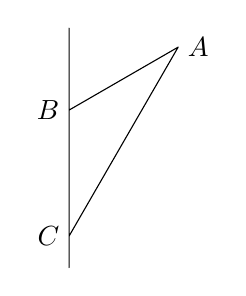
\begin{tikzpicture}[line cap=round,line join=round,scale=0.8]        
      \draw (1.732,1) coordinate (A) node[right] {$A$}
            (0,0) coordinate (B) node[left] {$B$}
            (0,-2) coordinate (C) node[left] {$C$};
      
      \draw (B)--(A)--(C) (0,-2.5)--(0,1.3);
      \end{tikzpicture}
      \caption{}\label{fig-190705-1930}
    \end{minipage}
    \hskip 0.5cm  
    \begin{minipage}[b]{0.45\linewidth}
      \centering
      \begin{tikzpicture}[line cap=round,line join=round,scale=1.3]
      \draw (0,0,0) coordinate (A) node[left] {$A$}
            ({2*sin(60)},0,{2*cos(60)}) coordinate (B) node[below] {$B$}
            (2,0,0) coordinate (C) node[right] {$C$}
            (A)++(0,2,0) coordinate (A1) node[left] {$A_1$}
            (A1)++(B) coordinate (B1) node[anchor=north west] {$B_1$}
            (A1)++(C) coordinate (C1) node[right] {$C_1$}
            ($(A1)!0.5!(C1)$) coordinate (E) node[above] {$E$}
            ($(B)!0.5!(C)$) coordinate (F) node[anchor=north west] {$F$};
      
      \draw (F)--(C1)--(C)--(B)--(B1)--(C1)--(A1)--(B1) (A1)--(A)--(B);
      \draw[densely dashed] (B)--(E)--(A)--(C)--(E)--(B); 
      \end{tikzpicture}
      \caption{}\label{fig-190705-1940}
    \end{minipage}
    \end{figure}

\lianxi
\begin{exercise}[s]
    某长方体的长、宽、高分别为 $\sqrt3$,$\sqrt2$,$1$, 求其外接球的表面积.
\end{exercise}
\beginsolution
    长方体的体对角线长
    \[\sqrt{(\sqrt3)^2+(\sqrt2)^2+1^2}= \sqrt6,\]
    也是外接球的直径, 故外接球的半径 $r= \dfrac{\sqrt6}2$, 表面积为
    \[4\pi r^2= 4\pi\Bigl(\frac{\sqrt6}2\Bigr)^2= 6\pi.\]
\endsolution

\subsubsection{求几何体的体积}
\begin{example}
    如图 \ref{fig-190705-1940} 所示, 在直三棱柱 $ABC\text{--}A_1 B_1 C_1$ 中, $AB\perp BC$, $AA_1 =AC=2$, $BC=1$, $E$,$F$ 分别为 $A_1 C_1$,$BC$ 的中点.
    
    (1) 求证: 平面 $ABE\perp$ 平面 $B_1 BCC_1$;
    
    (2) 求证: $C_1 F\parallel $ 平面 $ABE$;
    
    (3) 求三棱锥 $E\text{--}ABC$ 的体积.
\end{example}
\beginsolution
    (1) 由题意, $BB_1\perp AB$, 而 $AB\perp BC$, 所以 $AB\perp$ 平面 $B_1 BCC_1$, 则平面 $ABE\perp$ 平面 $B_1 BCC_1$.

    (2) 取 $AB$ 中点 $G$, 连接 $GE$,$GF$. 因为 $E$,$F$ 分别为 $A_1 C_1$,$BC$ 的中点, 所以
    \[GF\parallel AC\parallel EC_1,\quad
        GF= \frac12 AC= \frac12 A_1C_1= EC_1,\]
    表明四边形 $FGEC_1$ 为平行四边形, 因此 $C_1F\parallel EG$, 则 $C_1 F\parallel $ 平面 $ABE$.

    (3) 由题意, 三棱锥 $E\text{--}ABC$ 与直三棱柱 $ABC\text{--}A_1 B_1 C_1$ 同底等高. 因为 $AB\perp BC$, $AC=2$, $BC=1$, 所以 $AB=\sqrt3$, $\triangle ABC$ 的面积
    \[S_{\triangle ABC}= \frac12 AB\cdot BC= \frac{\sqrt3}2.\]
    又因为 $AA_1= 2$, 所以三棱锥 $E\text{--}ABC$ 的体积
    \[V_{E\text{--}ABC}= \frac13 S_{\triangle ABC}\cdot AA_1
        = \frac{\sqrt3}3.\]
\endsolution
    
\lianxi
\begin{exercise}[s]
    如图 \ref{fig-190708-1100} 所示, 在三棱锥 $A\text{--}BCD$ 中, $AB\perp$ 平面 $BCD$, $CD\perp BD$.
    
    (1) 求证: $CD\perp$ 平面 $ABD$;\qquad
    (2) 若 $AB=BD=CD=1$, $M$ 为 $AD$ 的中点, 求三棱锥 $A\text{--}MBC$ 的体积.
\end{exercise}
\beginsolution
    (1) 因为 $AB\perp$ 平面 $BCD$, 所以 $AB\perp CD$, 结合 $CD\perp BD$ 知 $CD\perp$ 平面 $ABD$.

    (2) 由题意, 底面 $\triangle BCD$ 的面积为 $\dfrac12 CD\cdot BD= \dfrac12$, 而 $M$ 为 $AD$ 的中点, 所以三棱锥 $A\text{--}MBC$ 的体积为三棱锥 $A\text{--}BCD$ 的体积的一半. 由 $AB\perp$ 平面 $BCD$ 知所求体积为
    \[\frac12\cdot \frac13\cdot S_{\triangle BCD}\cdot AB
        = \frac1{12}.\]
\endsolution

    \begin{figure}[htb]
    \small
    \centering
    \begin{minipage}[b]{0.45\linewidth}
      \centering
      \begin{tikzpicture}[line cap=round,line join=round,scale=2]        
      \draw (0,1,0) coordinate (A) node[left] {$A$}
            (0,0,0) coordinate (B) node[left] {$B$}
            (1,0,1) coordinate (C) node[below] {$C$}
            (1,0,0) coordinate (D) node[right] {$D$}
            ($(A)!0.5!(D)$) coordinate (M) node[anchor=south west] {$M$};
      
      \draw (A)--(B)--(C)--(A)--(D)--(C)--(M);
      \draw[densely dashed] (M)--(B)--(D);
      \end{tikzpicture}
      \caption{}\label{fig-190708-1100}
    \end{minipage}
    \hskip 0.5cm  
    \begin{minipage}[b]{0.45\linewidth}
      \centering
      \begin{tikzpicture}[line cap=round,line join=round,scale=1]
      \draw (0,0,0) coordinate (A) node[left] {$A$}
            (2,0,0) coordinate (B) node[right] {$B$}
            (0.8,0,-2) coordinate (C) +(0,0.1,0) node[left] {$C$}
            (A)++(0,2.3,0) coordinate (A1) node[left] {$A_1$}
            (B)++(A1) coordinate (B1) node[right] {$B_1$}
            (C)++(A1) coordinate (C1) node[above] {$C_1$}
            ($(A1)!0.5!(B1)$) coordinate (D) node[above] {$D$}
            ($(A1)!0.5!(A)$) coordinate (E) node[left] {$E$}
            ($(A)!0.25!(B)$) coordinate (F) node[below] {$F$}
            ($(A)!0.5!(C)$) coordinate (G) +(0,-0.1,0) node[right] {$G$};
      
      \draw (B)--(A)--(A1)--(B1)--(B)--(D)--(C1)--(B1) (C1)--(A1) (E)--(F);
      \draw[densely dashed] (A)--(C)--(B)--(C1)--(C) (E)--(G)--(F); 
      \end{tikzpicture}
      \caption{}\label{fig-190708-1110}
    \end{minipage}
    \end{figure}
     
\subsubsection{几何体的体积探索问题}
\begin{example}
    如图 \ref{fig-190708-1120} 所示, 在四棱锥 $P\text{--}ABCD$ 中, 四边形 $ABCD$ 为矩形, 平面 $PAD\perp$ 平面 $ABCD$.
    
    (1) 求证: $AB\perp PD$;\qquad
    (2) 若 $\angle BPC=90^\circ$, $PB=\sqrt2$, $PC=2$, 则当 $AB$ 为何值时, 四棱锥 $P\text{--}ABCD$ 的体积最大\,?
\end{example}
\beginsolution
    (1) 因为四边形 $ABCD$ 为矩形, 所以 $AB\perp AD$, 结合 平面 $PAD\perp$ 平面 $ABCD$ 知 $AB\perp$ 平面 $PAD$, 则 $AB\perp PD$.

    (2) 过点 $P$ 作 $PE\perp AD$ 于点 $E$, 连接 $EB$,$EC$. 因为平面 $PAD\perp$ 平面 $ABCD$, 所以 $PE\perp$ 平面 $ABCD$, 则 $PE$ 为四棱锥 $P\text{--}ABCD$ 的高, 且 $PE\perp EB$, $PE\perp EC$. 
    
    \mymarginpar{过点 $E$ 作 $EF\perp AD$ 于点 $E$, 交 $BC$ 于点 $F$, 连接 $PF$, 则可证 $\angle PEF= 90^\circ$, $EF=AB= a$, $PF= \dfrac2{\sqrt3}$, 也可得 $h^2+a^2= \dfrac43$.}
    设 $PE=h$, $AB= a$, $AE= l$. 因为 $\angle BPC=90^\circ$, $PB=\sqrt2$, $PC=2$, 所以
    \[AV= BC= \sqrt6,\quad DE= AD-AE= \sqrt6-l.\]
    在 $\mathrm{Rt}\triangle PEB$ 和 $\mathrm{Rt}\triangle PEC$ 中,
    \[PE^2+ EC^2= PC^2,\quad PE^2+ EB^2= PB^2,\]
    则
    \[\left\{\!\!\begin{array}{l}
        h^2+ (\sqrt6-l)^2+ a^2= 4,\\
        h^2+ l^2+ a^2= 2,
    \end{array}\right.\]
    作差得 $l= \dfrac{\sqrt6}3$, 而 $h^2+a^2= \dfrac43$.

    四棱锥 $P\text{--}ABCD$ 的体积
    \[V_{P\text{--}ABCD}= \frac13 AB\cdot AD\cdot PE
        = \frac{\sqrt6}3 ah.\]
    因为 $h^2+a^2\geqslant 2ah$, 所以 
    \[ah\leqslant \frac23,\quad
        \frac{\sqrt6}3 ah\leqslant \frac{2\sqrt6}9,\]
    等号成立当且仅当 $a=h=\dfrac{\sqrt6}3$. 所以当 $AB= \dfrac{\sqrt6}3$ 时, 四棱锥 $P\text{--}ABCD$ 的体积最大.
\endsolution

\lianxi
\begin{exercise}[s]
    如图 \ref{fig-190708-1110} 所示, 在三棱柱 $ABC\text{--}A_1 B_1 C_1$ 中, $AA_1 \perp$ 平面 $ABC$, $D$, $E$ 分别为 $A_1 B_1$, $AA_1$ 的中点, 点 $F$ 在棱 $AB$ 上, 且 $AF=\dfrac14 AB$.
    
    (1) 求证: $EF\parallel$ 平面 $BDC_1$.\qquad
    (2) 在棱 $AC$ 上是否存在一个点 $G$, 使得平面 $EFG$ 
    将三棱柱分割成的两部分体积之比为 $1:15$?
\end{exercise}
\beginsolution
    (1) 取 $AB$ 中点 $H$, 连接 $AH$. 因为 $D$ 为 $A_1B_1$ 的中点, 四边形 $ABB_1A_1$ 为平行四边形, 所以 $A_1D\parallel HB$, $A_1D= HB$, 即四边形 $A_1HBD$ 也为平行四边形, 则 $A_1H\parallel BD$. 又因为 $E$ 为 $AA_1$ 的中点, $AF= \dfrac14 AB$, 所以 $EF\parallel A_1H$, 则 $EF\parallel BD$, 表明 $EF\parallel$ 平面 $BDC_1$.

    (2) 三棱锥 $E\text{--}AFG$ 与三棱柱 $ABC\text{--}A_1 B_1 C_1$ 的体积之比为
    \[\frac13\cdot \frac{AF}{AB}\cdot \frac{AG}{AC}
        \cdot \frac{AE}{AA_1}= \frac{AG}{24AC}.\]
    若满足题意的点 $G$ 存在, 则上述比值为 $\dfrac1{16}$, 即
    \[\frac{AG}{24AC}= \frac1{16},\quad 
        \frac{AG}{AC}= \frac32.\]
    此时 $AG>AC$, 即点 $G$ 在棱 $AC$ 的延长线上, 与题意不合, 故不存在满足题意的点 $G$.
\endsolution

    \begin{figure}[htb]
    \small
    \centering
    \begin{minipage}[b]{0.45\linewidth}
      \centering
      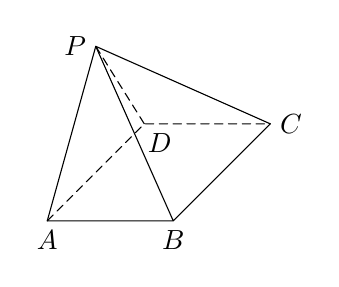
\begin{tikzpicture}[line cap=round,line join=round,scale=1.6]        
      \draw (0,0,0) coordinate (D) +(-0.05,0,0) node[anchor=north west] {$D$}
            (0,0,2) coordinate (A) node[below] {$A$}
            (1,0,0) coordinate (C) node[right] {$C$}
            (A)++(C) coordinate (B) node[below] {$B$}
            (0,1,1) coordinate (P) node[left] {$P$};
      
      \draw (P)--(A)--(B)--(P)--(C)--(B);
      \draw[densely dashed] (A)--(D)--(C) (P)--(D);
      \end{tikzpicture}
      \caption{}\label{fig-190708-1120}
    \end{minipage}
    \hskip 0.5cm  
    \begin{minipage}[b]{0.45\linewidth}
      \centering
      \begin{tikzpicture}[line cap=round,line join=round,scale=1.2]
      \draw (0,0,0) coordinate (A) node[left] {$A$}
            (1,0,1.7) coordinate (B) node[below] {$B$}
            (2,0,0) coordinate (C) node[right] {$C$}
            (1,1.8,0.5) coordinate (P) node[left] {$P$}
            ($(P)!0.5!(B)$) coordinate (D) +(0,0.1,0) node[anchor=south west] {$D$}
            ($(P)!0.5!(C)$) coordinate (E) node[right] {$E$};
      
      \draw (A)--(B)--(C)--(P)--(A)--(D)--(E)--(B)--(P);
      \draw[densely dashed] (C)--(A)--(E); 
      \end{tikzpicture}
      \caption{}\label{fig-190708-1130}
    \end{minipage}
    \end{figure}

\subsubsection{课堂评价}
\begin{exercise}
    已知正方形 $ABCD$ 的边长为 $2$, $E$, $F$ 分别为 $BC$, $DC$ 的中点, 沿 $AE$,$EF$,$AF$ 折成一个四面体, 使 $B$,$C$,$D$ 三点重合, 求这个四面体的体积.
\end{exercise}
\beginsolution
    翻折后, $AB\perp BE$, $AB\perp BF$, 则 $AB$ 为三棱锥 $A\text{--}BEF$ (即题中的四面体) 的高, 故所求体积为
    \[\frac13S_{\triangle BEF}\cdot AB= \frac13.\]
\endsolution

\begin{exercise}
    如图 \ref{fig-190708-1130} 所示, 在三棱锥 $P\text{--}ABC$ 中, $D$,$E$ 分别为 $PB$,$PC$ 的中点, 记三棱锥 $D\text{--}ABE$ 的体积为 $V_1$, 三棱锥 $P\text{--}ABC$ 的体积为 $V_2$, 求 $\dfrac{V_1}{V_2}$ 的值.
\end{exercise}
\beginsolution
    三棱锥 $D\text{--}ABE$ 可视为三棱锥 $A\text{--}BDE$, 它与三棱锥 $A\text{--}PBC$ 同底等高, 所以
    \[\dfrac{V_1}{V_2}
        = \frac{S_{\triangle BDE}}{S_{\triangle PBC}}
        = \frac 14.\]
\endsolution
    
\begin{exercise}
    在如图 \ref{fig-190708-1140} 所示的几何体中, 平面 $ACE\perp$ 平面 $ABCD$, 四边形 $ABCD$ 为平行四边形, $\angle ACB=90^\circ$, $EF\parallel BC$, $AC=BC=\sqrt2$, $AE=EC=1$.
    
    (1) 求证: $AE\perp$ 平面 $BCEF$;\qquad
    (2) 求三棱锥 $D\text{--}ACF$ 的体积.
\end{exercise}
\beginsolution
    (1) 因为 $\angle ACB=90^\circ$, 平面 $ACE\perp$ 平面 $ABCD$, 所以 $BC\perp$ 平面 $ACE$, 则 $BC\perp AE$. 由  $AC=\sqrt2$, $AE=EC=1$ 知,
    \[AC^2= AE^2+EC^2,\quad\text{即}\quad 
        \angle AEC= 90^\circ,\]
    所以 $AE\perp EC$. 因为 $EF\parallel BC$, 所以 $B$,$C$,$E$,$F$ 共面, 则 $AE\perp$ 平面 $BCEF$.

    (2) 三棱锥 $D\text{--}ACF$ 也可视为三棱锥 $F\text{--}ACD$. 由 $EF\parallel BC$ 知, 该三棱锥与三棱锥 $E\text{--}ACD$ 体积相同. 过点 $E$ 作 $EG\perp AC$ 于点 $G$. 由平面 $ACE\perp$ 平面 $ABCD$ 知, $EG\perp$ 平面 $ABCD$, 则 $EG$ 为三棱锥 $E\text{--}ACD$ 的高. 因为 $AC=\sqrt2$, $AE=EC=1$, 所以 $\triangle AEC$ 为等腰直角三角形, $EC= \dfrac{\sqrt2}2$. 又因为四边形 $ABCD$ 为平行四边形, $\angle ACB= 90^\circ$, $BC=\sqrt2$, 所以 $\triangle ACD$ 的面积
    \[S_{\triangle ACD}= S_{\triangle ACB}
        = \frac12AC\cdot BC= 1,\]
    则三棱锥 $E\text{--}ACD$ 的体积
    \[V_{E\text{--}ACD}= \frac13S_{\triangle ACD}\cdot EG
        = \frac{\sqrt2}6,\]
    即三棱锥 $D\text{--}ACF$ 的体积也为 $\dfrac{\sqrt2}6$.
\endsolution

    \begin{figure}[htb]
    \small
    \centering
    \begin{minipage}[b]{0.45\linewidth}
      \centering
      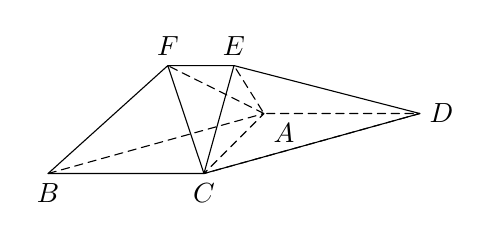
\begin{tikzpicture}[line cap=round,line join=round,scale=1.4]        
      \draw (0,0,0) coordinate (A) node[anchor=north west] {$A$}
            (0,0,1.414) coordinate (C) node[below] {$C$}
            (-1.414,0,1.414) coordinate (B) node[below] {$B$}
            (1.414,0,0) coordinate (D) node[right] {$D$}
            (0,0.707,0.707) coordinate (E) node[above] {$E$}
            (E)++(-0.6,0,0) coordinate (F) node[above] {$F$};
      
      \draw (F)--(B)--(C)--(F)--(E)--(C)--(D)--(E);
      \draw[densely dashed] (B)--(A)--(C)--(D)--(A)--(E) (A)--(F);
      \end{tikzpicture}
      \caption{}\label{fig-190708-1140}
    \end{minipage}
    \hskip 0.5cm  
    \begin{minipage}[b]{0.45\linewidth}
        \centering
        \begin{tikzpicture}[line cap=round,line join=round,scale=1.4]        
        \draw (0,0,0) coordinate (O) node[below] {$O$}
              ({sin(-45)},0,{cos(-45)}) coordinate (A) node[below] {$A$}
              ({sin(45)},0,{cos(45)}) coordinate (B) node[below] {$B$}
              ({sin(135)},0,{cos(135)}) coordinate (C) node[right] {$C$}
              ({sin(225)},0,{cos(225)}) coordinate (D) +(0,-0.05,0) node[below] {$D$}
              (0,1.2,0) coordinate (A1) node[left] {$A_1$}
              ($(A1)+(B)-(A)$) coordinate (B1) +(0.15,0,0) node[right] {$B_1$}
              ($(A1)+(C)-(A)$) coordinate (C1) node[right] {$C_1$}
              ($(A1)+(D)-(A)$) coordinate (D1) node[left] {$D_1$};
        
        \draw (C)--(B)--(A)--(A1)--(B)--(B1)--(A1)--(D1)--(B1)--(C1)--(D1) (B1)--(C)--(C1);
        \draw[densely dashed] (A)--(D)--(A1) (C)--(D)--(D1) (B)--(D) (A1)--(O);
        \end{tikzpicture}
        \caption{}\label{fig-190708-1740}
      \end{minipage}
    \end{figure}
    
\subsection{课后练习}  
\begin{exercise}
    若正四棱锥的底面边长为 $6$, 高为 $\sqrt7$, 求这个正四棱锥的侧面积.
\end{exercise}
\beginsolution
    作图易知, 该正四棱锥的四个侧面均为等腰三角形, 且底为 $6$, 高为 $\sqrt{(\sqrt7)^2+3^2}= 4$, 所以侧面积为
    \[4\cdot \frac12\cdot 4\cdot 6= 48.\]
\endsolution

\begin{exercise}
    以边长为 $1$ 的正方形的一边所在直线为旋转轴, 将该正方形旋转一周, 求所得几何体的侧面积. 若绕该正方形的一条对角线所在直线旋转, 求对应几何体的侧面积.
\end{exercise}
\beginsolution
    若绕一边旋转, 则得到圆柱, 且底面半径和高均为 $1$, 所以侧面积为
    \[2\pi\cdot 1\cdot 1= 2\pi.\]

    若绕一条对角线旋转, 则得到两个圆锥, 且底面半径和高均为 $\dfrac{\sqrt2}2$, 母线长为 $1$, 所以侧面积为
    \[2\pi\cdot \frac{\sqrt2}2\cdot 1= \sqrt2\pi.\]
\endsolution

\begin{exercise}
    四棱锥 $P\text{--}ABCD$ 的底面是正方形, $PD\perp$ 底面 $ABCD$, 点 $E$ 在棱 $PB$ 上. 若 $PD=\sqrt2 AB=2$, 且三棱锥 $A\text{--}PED$ 的体积 $V_{A\text{--}PED}=\dfrac13$, 求 $\dfrac{PE}{EB}$ 的值.
\end{exercise}
\beginsolution
    连接 $BD$, 由题意, 三棱锥 $P\text{--}ABD$ 的体积是四棱锥 $P\text{--}ABCD$ 的一半, 即
    \[V_{P\text{--}ABD}= \frac12V_{P\text{--}ABCD}
        = \frac12\cdot \frac13 PD\cdot AD\cdot AB
        = \frac23.\]
    由 $V_{A\text{--}PED}= \dfrac13= \frac12 V_{P\text{--}ABD}$ 知, $E$ 为 $PB$ 的中点, 即 $\dfrac{PE}{EB}=1$.
\endsolution

\begin{exercise}
    如图 \ref{fig-190708-1740} 所示, 四棱柱 $ABCD\text{--}A_1 B_1 C_1 D_1$ 的底面 $ABCD$ 是正方形, 点 $O$ 是底面的中心, $A_1 O\perp$ 底面 $ABCD$, $AB=AA_1 =\sqrt2$.
    
    (1) 求证: 平面 $A_1 BD\parallel$ 平面 $CD_1 B_1$;
    
    (2) 求三棱柱 $ABD\text{--}A_1 B_1 D_1$ 的体积.
\end{exercise}
\beginsolution
    (1) 在四棱柱 $ABCD\text{--}A_1 B_1 C_1 D_1$ 中,
    \[A_1B_1\parallel AB\parallel DC,\quad
        A_1B_!= AB= DC,\]
    所以四边形 $A_1DCB_1$ 为平行四边形, 则 $A_1D\parallel B1C$. 同理可证 $DB\parallel D_1B_1$, 所以平面 $A_1 BD\parallel$ 平面 $CD_1 B_1$.

    (2) 连接 $AO$. 因为点 $O$ 是正方形 $ABCD$ 的中心, 而 $AB=\sqrt2$, 所以 $AO=1$. 而 $A_1O\perp $ 底面 $ABCD$, $A_1A=\sqrt2$, 所以 $A_1O=1$, 且 $A_1O$ 为三棱锥 $ABD\text{--}A_1B_1D_1$ 的高. 由 $\triangle ABD$ 的面积
    \[S_{\triangle ABD}= \frac12 AB\cdot AD= 1\]
    可知, 三棱柱 $ABD\text{--}A_1 B_1 D_1$ 的体积
    \[V_{ABD\text{--}A_1 B_1 D_1}
        = S_{\triangle ABD}\cdot A_1O= 1.\]
\endsolution

\begin{exercise}
    如图 \ref{fig-190708-1750}, 在矩形 $ABCD$ 中, 对角线 $AC$, $BD$ 的交点为 $G$, $AD\perp$ 平面 $ABE$, $AE\perp EB$, $AE=EB=BC=2$, 且 $BF\perp CE$ 于点 $E$.
    
    (1) 求证: $AE\perp$ 平面 $BCE$;\qquad
    (2) 求证: $AE\parallel$ 平面 $BFD$;
    
    (3) 求三棱锥 $C\text{--}GBF$ 的体积.
\end{exercise}
\beginsolution
    (1) 因为 $AD\perp$ 平面 $ABE$, 在矩形 $ABCD$ 中, $AD\parallel BC$, 所以 $BC\perp$ 平面 $ABE$, 则 $BC\perp AE$. 由 $AE\perp EB$ 知, $AE\perp$ 平面 $BCE$.

    (2) 因为 $EB=BC=2$, $BF\perp CE$, 所以 $F$ 为 $EC$ 中点. 在矩形 $ABCD$ 中, $G$ 为 $AC$ 中点, 所以 $AE\parallel GF$, 则 $AE\parallel$ 平面 $BFD$.

    (3) 取 $AB$ 中点 $H$, 连接 $EH$. 因为 $AE=EB=2$, $AE\perp EB$, 所以 $EH\perp AB$, $AB= 2\sqrt2$ 且 $EH=\sqrt2$. 由 $AD\perp$ 平面 $ABE$ 知, 平面 $ABCD\perp$ 平面 $ABE$, 所以 $EH\perp$ 平面 $ABCD$. 结合 $F$ 为 $EC$ 中点可知, 点 $F$ 到平面 $ABCD$ 的距离为 $\dfrac12 EH$. 在矩形 $ABCD$ 中, $\triangle BCG$ 的面积
    \[S_{\triangle BCG}= \frac14 S_{ABCD}= \sqrt2,\]
    所以三棱锥 $F\text{--}BCF$ 的体积
    \[V_{F\text{--}BCF}
        = \frac13 S_{\triangle BCG}\cdot \frac12 EH
        = \frac13,\]
    即三棱锥 $C\text{--}GBF$ 的体积为 $\dfrac13$.
\endsolution
        
    \begin{figure}[htb]
    \small
    \centering
    \begin{minipage}[b]{0.45\linewidth}
      \centering
      \begin{tikzpicture}[line cap=round,line join=round,scale=1]
      \draw (0,0,0) coordinate (A) node[left] {$A$}
            (2.828,0,0) coordinate (B) node[right] {$B$}
            (0,2,0) coordinate (D) node[left] {$D$}
            (B)++(D) coordinate (C) node[right] {$C$}
            (1,0,2) coordinate (E) node[below] {$E$}
            ($(E)!0.5!(C)$) coordinate (F) node[below] {$F$}
            ($(A)!0.5!(C)$) coordinate (G) node[above] {$G$};
      
      \draw (C)--(D)--(A)--(E)--(B)--(C)--(E)--(D)--(F)--(B);
      \draw[densely dashed] (C)--(A)--(B)--(D) (F)--(G); 
      \end{tikzpicture}
      \caption{}\label{fig-190708-1750}
    \end{minipage}
    \hskip 0.5cm
    \begin{minipage}[b]{0.45\linewidth}
        \centering
        \begin{tikzpicture}[line cap=round,line join=round,scale=0.3]
        \draw (-4,0,4) coordinate (A) node[below] {$A$}
              (4,0,4) coordinate (B) node[below] {$B$}
              (4,0,-4) coordinate (C) node[right] {$C$}
              (-4,0,-4) coordinate (D) +(0.1,0,0) node[below] {$D$}
              (0,6,0) coordinate (P) node[left] {$P$}
              ($(A)!0.75!(B)$) coordinate (E) node[below] {$E$}
              ($(D)!0.75!(C)$) coordinate (F) node[below] {$F$}
              ($(P)!0.5!(B)$) coordinate (G) node[left] {$G$}
              ($(P)!0.5!(C)$) coordinate (H) node[anchor=south west] {$H$};
        
        \draw (P)--(A)--(B)--(P)--(C)--(B) (E)--(G)--(H);
        \draw[densely dashed] (A)--(D)--(P) (D)--(C) (E)--(F)--(H); 
        \end{tikzpicture}
        \caption{}\label{fig-190708-1150}
      \end{minipage}
    \end{figure}

\begin{exercise}
    如图 \ref{fig-190708-1150} 所示, 正四棱锥 $P\text{--}ABCD$ 的底面是边长为 $8$ 的正方形, 四条侧棱长均为 $2\sqrt{17}$, 点 $G$,$E$,$F$,$H$ 分别是棱 $PB$,$AB$,$CD$,$PC$ 上共面的四点, 且平面 $GEFH\perp$ 平面 $ABCD$, $BC\parallel$ 平面 $GEFH$.
    
    (1) 求证: $GH\parallel EF$;
    
    (2) 若 $EB=2$, 求几何体 $BEG\text{--}CFH$ 的体积.
\end{exercise}
\beginsolution
    (1) 因为 $BC\parallel$ 平面 $GEFH$, 所以 $BC\parallel EF$, $BC\parallel GH$, 则 $GH\parallel EF$.

    (2) 作点 $P$ 在平面 $ABCD$ 上的射影, 记为点 $O$, 则 $O$ 为正方形 $ABCD$ 的中心, 连接 $AO$. 由题意, $AO=4\sqrt2$, $AP= 2\sqrt{17}$, 所以
    \[PO= \sqrt{AP^2- AO^2}= 6,\]
    即正四棱锥 $P\text{--}ABCD$ 的高为 $6$.

    取 $AD$ 中点 $I$, 连接 $PI$. 由 $BE=2$ 可证 $G$,$H$ 分别为 $PB$,$PC$ 中点, 连接 $HB$,$HE$. 分别计算四棱锥 $H\text{--}EBCF$ 和三棱锥 $B\text{--}EGH$ 的体积, 可知几何体 $BEG\text{--}CFH$ 的体积为 $16+4= 20$.
\endsolution